\section{Applications}
\label{ch:app}

\epigraph{Simplicity is complicated.}{Rob Pike}

In this chapter, we first introduce a possible application of our proposed model.
This includes the implemented features, how the model could benefit a user, 
as well as the architecture and data flow of the application.
In the second part of this chapter, we formalize and discuss 
the possibilities and benefits of being a standard web API for web developers 
and website designer.

\subsection{Client-side Browser Plugin}
\label{sec:plugin}

We developed a client-side browser plugin as a illustration of our model application.
The plugin is an intelligent system that proactively serves its user
and provides proactive notifications based on the historical actions in a session
when browsing behavior is detected to goal-oriented or fuzzy behavior, 
as illustrated in Figure \ref{fig:proactive-noti}.

The user can either select ``Yes'' and navigate to the most likely page that they 
will visit in the future, or select ``No'' to ignore the notification and mark it as an invalid detection.
The plugin serves the user only if the browsing behavior is clearly detected 
to forbear massive notification that disturb the user. 
We argue that the plugin is only a supplement for improving
browsing experience but is not always necessary. For instance in exploring behavior, 
a user's information need may not be clearly observed and the recommendations may not 
useful. 
One of the benefits of the plugin is to proactively help the user become efficient
and reach the destination as fast as possible in the goal-oriented browsing.

\begin{figure}[H]
    \centering
    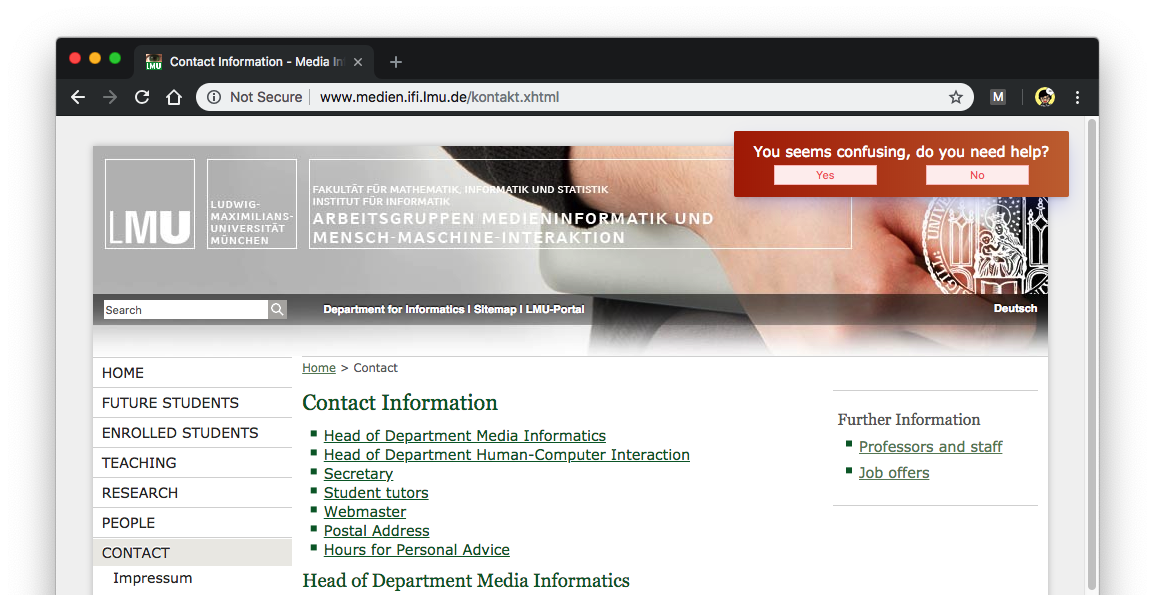
\includegraphics[width=0.7\textwidth]{figures/proactive-noti}
    \caption{Proactive notification:
    The plugin injects monitor script when the page is loaded, and then serve user giving
    notification when detecting fuzzy browsing behavior.}
    \label{fig:proactive-noti}
\end{figure}

\begin{figure}
    \centering
    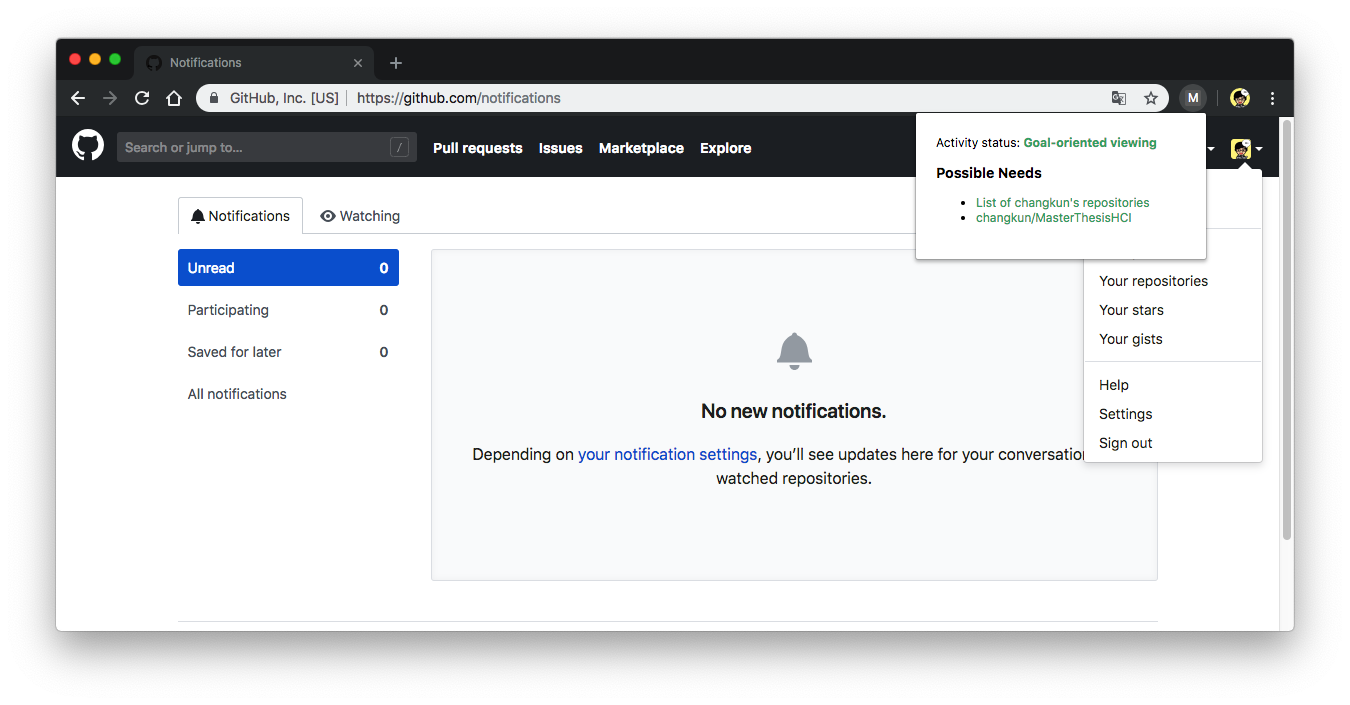
\includegraphics[width=0.7\textwidth]{figures/plugin-predicting-result}
    \caption{The plugin provided popup page: users can always open the page
    to understand the current status of browsing and predicted needs based on
    historical actions in a browsing session. In this case, the detected browsing behavior
    is under a goal-oriented browsing, and predicted actions
    are accessing the page of public GitHub repositories and accessing a specific repository.}
    \label{fig:plugin-predict}
\end{figure}

In Figure \ref{fig:plugin-predict}, other than proactive notification, 
users can always open a popup page provided by the plugin.
The popup page enables another interaction that privides the predicted needs 
based on historical user actions. A user can always interact with the plugin and
retrieve the possible needs and browsing status in the current session.
This information is helpful to the plugin user because a user can understand
the current status of web browsing, which implicitly allows the person to better focus
on whether the person is detected as a form of exploring browsing behavior.

The implementation and architecture is not simple
although it provides a small feature that exhibits context and future information for the user.
Figure \ref{fig:arch} illustrates the implemented architecture of the plugin.

First of all, the plugin daemon process will inject monitoring script (\emph{step2}) intoto 
the newly opened page (\emph{step1}).
When the user starts browsing and interacting (\emph{step3}), the injected script will report the referring of
previous visited URL, current URL and stay duration to the daemon process of the plugin (\emph{step4}).

Afterwards, the daemon process will report the referring information to the plugin server webhook (\emph{step5}).
Next, the webhook will immediately request the intra prediction microservice (\emph{step6}) and result in a 
prediction (\emph{step7}), which will then respond the prediction result to the daemon process 
with a pre-trained model (\emph{step8}). Therefore the daemon process can decide 
if a proactive notification should be presented to the user or whether it should simply update its popup page
for illustration (\emph{step9}).

Since the prediction service received a new user action, it stores the action into a database
subsequently for the model update (\emph{step10}). Because of the cost of training a new model,
the prediction service can decide to trigger the training service to retrain the model 
if it has already received enough new data (\emph{step11}).

\begin{figure}[H]
    \centering
    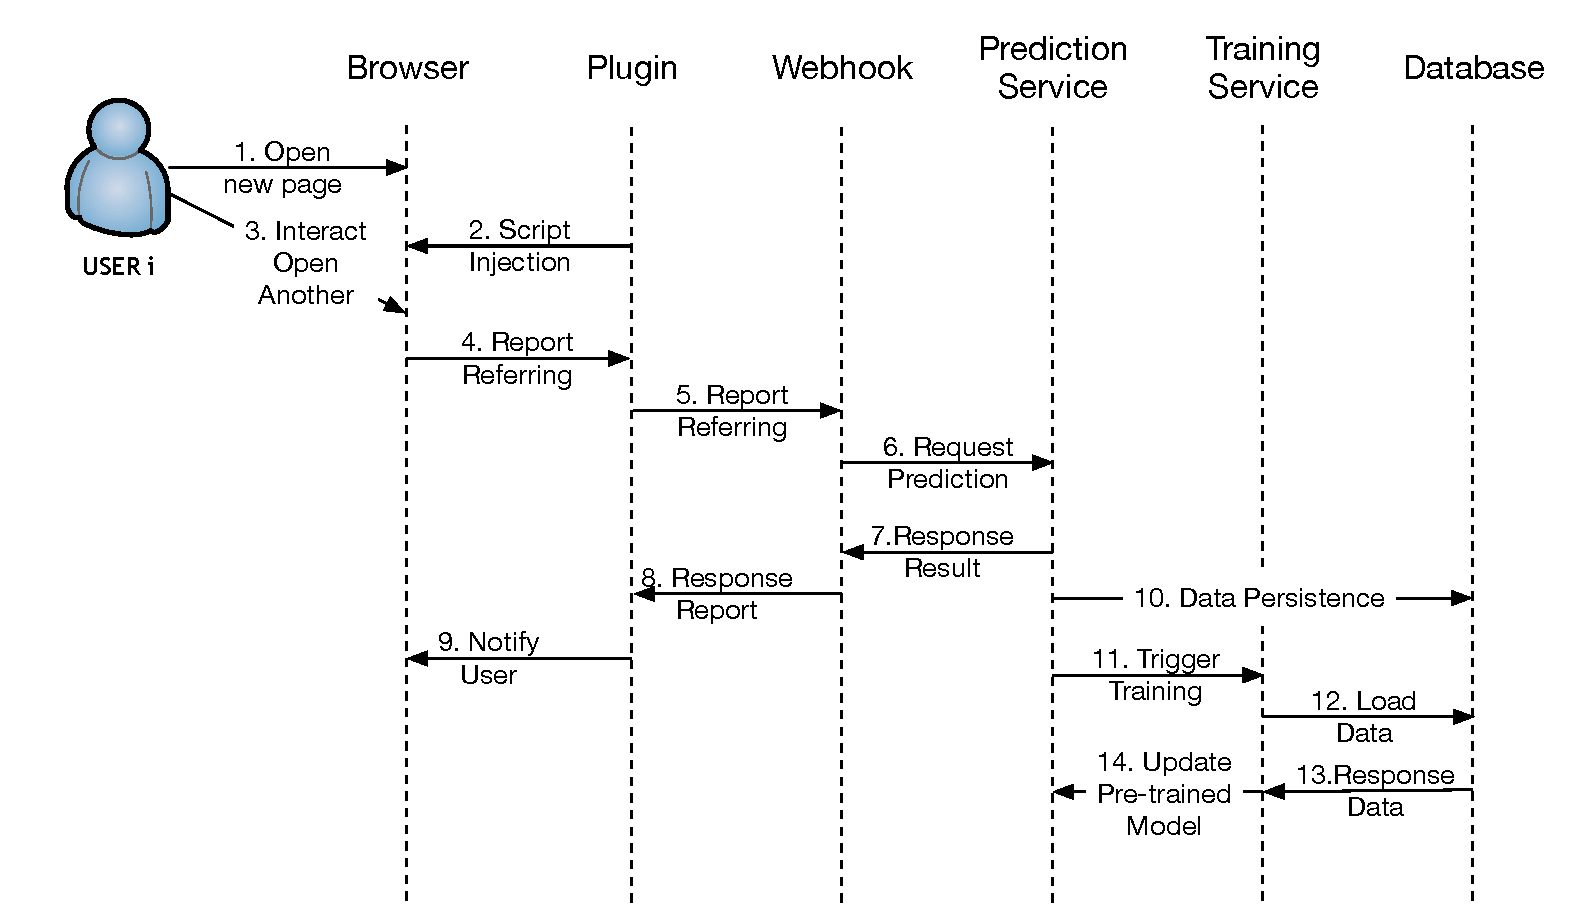
\includegraphics[width=0.7\textwidth]{figures/arch}
    \caption{The implemented architecture of our plugin: This is the data flow illustration,
    Step 1 and 3 are user actions, and the rest of the steps are automatically triggered by
    each component of the plugin. For instance, the browser deamon process
    and plugin background process as two part of client-side components, the webhook,
    prediction service and training service are backend microservices running on a server.}
    \label{fig:arch}
\end{figure}

Furthermore, the training service uses the pre-trained model as
a base model to initiate the training by requesting newly created data from database (\emph{step12} and \emph{step13}), 
similar to the idea of transfer learning.
After the training has achieved performance that is competitive to the pre-trained model,
the training service will update the newly trained model to the prediction service (\emph{step14}), which 
serves future prediction requests.

As we can observe from the architecture, the infrastructure is not as simple as 
the plugin feature intends to provide. Therefore, we argue that the plugin feature is a feature that
only browser manufacturers can provide. In the following section, we formalize and discuss 
the possibilities of the plugin feature as a web API.

\subsection{Web API Standardization and Platform-as-a-Service}

Web API is a generic term used in various fields of development.
Web API in the context of web browsers refer to the APIs provided
by browser manufacturers to developers that helps with web applications.
These APIs can even close
help with manipulating hardware, for instance, WebAssembly \cite{w3c2018ws}.

Currently, there are experimental standard web APIs such as web speech APIs \cite{mozilla2019speech}
that integrate complex features to web developers and only have 
Google Chrome (after version 24) support. 
The specification proposal was initiated by Google. According to 
the source code of Chromium Kernel, the APIs are implemented based on 
the speech recognition service provided by Google Cloud Platform 
\footnote{\url{https://github.com/chromium/chromium/blob/83928864c18362a4b0f84bad9bee4104f4655430/content/browser/speech/speech\_recognition\_engine.cc\#L35}, last accessed on January 03, 2019},
which indicates that browser APIs do not only privide interfaces to
the hardware but also access cloud platform services, i.e. Platform-as-a-Service integrated 
APIs.

The plugin that was illustrated in Section \ref{sec:plugin} can also be integrated as a PaaS API
that is embedded into web browsers, which simplifies the infrastructure of the plugin. 
Developers can simply call the standardized API to report current user actions and
obtain a response about current behavior status as well as the prediction of future movement or 
actions; see Figure \ref{fig:webapi} for the diagrams.

\begin{figure}[H]
    \centering
    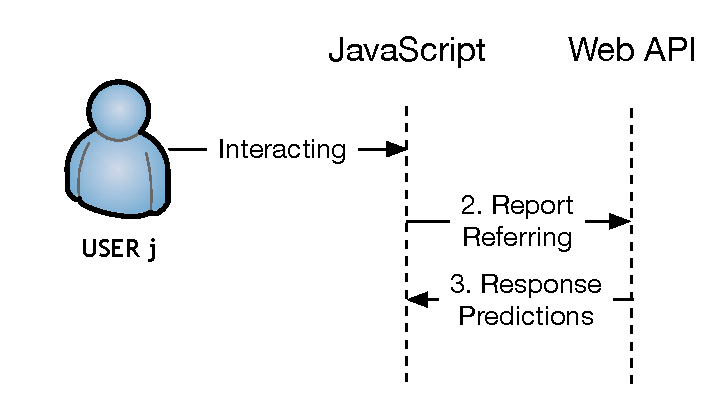
\includegraphics[width=0.4\textwidth]{figures/webapi}
    \caption{Usage overview of standadized BrowsingBehavior API}
    \label{fig:webapi}
\end{figure}

Defining the specification of the PaaS API aims enable web developers to
use a web browser to monitor the future actions of their users.
Developers can use the predicted actions to dynamically change the UI elements
and improve
the user experience of their product. 
We breifly discuss the non-normative web API design of the browsing behavior predictor,
which seeks to keep the API to a minimum. 

\subsubsection{The \emph{BrowsingBehavior} Interface}

The browsing behavior interface is a scripted web API for resulting in a monitored browsing
session, which is presented in Code \ref{lst:interface}.

\begin{lstlisting}[
    language={JavaScript},
    caption={BrowsingBehavior Interface},
    label={lst:interface}
]
[Exposed=Window, Constructor]
interface BrowsingBehavior : EventTarget {
    
    // methods to drive browsing behavior response
    void start();
    void stop();
    void pause();
    void resume();

    // event methods
    attribute EventHandler onBrowsingStart;
    attribute EventHandler onBrowsingEnd;
    attribute EventHandler onBrowsingPause;
    attribute EventHandler onBrowsingResume;
    attribute EventHandler onResult;
}
\end{lstlisting}

% self-reviewed afterwards

\paragraph{\emph{start()} method} When the start method is called, it represents the moment in
time the web application wishes to begin monitoring user's actions.
Then every step when a user was making moves, the \emph{EventHandler onResult} will produce
a standard prediction and classification of user browsing behavior. Further, 
the \emph{EventHandler onBrowsingStart} will be called immediately after calling 
this method and before resulting a prediction result, which gives a barrier in between of
calling \emph{start} and callback \emph{onResult}.

\paragraph{\emph{stop()} method} When the stop method is called, it represents the instruction
to browsing behavior service to stop monitoring user actions, and resulting in a 
final prediction in the \emph{EventHandler onBrowsingEnd}.

\paragraph{\emph{pause()} method} This method is used to ignoring the upcoming user actions
to pauses the monitoring of user actions, and resulting in a prediction in the 
\emph{EventHandler onBrowsingPause}.

\paragraph{\emph{resume()} method} This method resumes the paused \emph{BrowsingBehavior}
object and recovers the monitoring of user actions. Before monitoring is fully recovered,
the \emph{EventHandler onBrowsingResume} will be called.

The primary consideration of designing these four methods is to restrict abuse of the APIs.
Similar to cookie, speech recognition APIs, a website should acquire an authorization from
their user; otherwise, the API cannot monitor any user actions on the web, which partially
solves the issue of privacy and security. We will discuss more concerns about the feature in
Chapter \ref{ch:discuss}.

\subsubsection{\emph{onResult} callback}

\emph{onResult} callback passes the prediction after the browser user acted.
The prediction result consists of two parts: behavior and future movements.

The \emph{behavior} attribute of the result object is a JSON object that contains 
confidence level, i.e., classification probability, and a enumerate \emph{category} attribute
that indicate a finite set of user browsing behaviors, i.e., goal-oriented, fuzzy or exploring.

\begin{lstlisting}[
    language={JavaScript},
    caption={Result object of onResult callback},
    label={lst:callback}
]
{
    "behavior": {
        "confidence": float64,
        "category": string,
    },
    "futures": [
        {
            "confidence": float64,
            "actions": array[string],
        },
        {
            "confidence": float64,
            "actions": array[string],
        },
        ...
    ]
}
\end{lstlisting}

The \emph{futures} attribute of the result object is an ordered JSON object that from the
highest \emph{confidence} to lowerest {confidence} and the \emph{confidence} is a floating
number from minimum 0 to maximum 1. Meanwhile, the \emph{actions} attribute in a 
JSON object of an item of \emph{futures} array is an array of possible actions of URLs that
ordered in chronologic order, the first element represents the next immediate action,
and the last element represents the final action in the session, as shown in Code \ref{lst:callback}.

\begin{lstlisting}[
    language={JavaScript},
    caption={Formation of browser collections},
    label={lst:collect}
]
{
    "device_id": string,
    "previous_url": string,
    "current_url": string,
    "stay_seconds": float64,
    "time": string
}
\end{lstlisting}

From the perspective of implementation, browser manufacturers collect data after developer
calls \emph{start()}.
In Code \ref{lst:collect}, each time when a user performs an action, including open a new page,
switch to another tab or backtrack to former page, will result in a JSON object that contains
\emph{device\_id} a unique identifier that represents the device, \emph{previous\_url} the previous
URL of the action, \emph{current\_url} the current URL of the action, \emph{stay\_seconds}
the stay duration of \emph{previous\_url} and \emph{time} string of the time of data creation.

% \subsubsection{Communication Protocol}

\cleardoublepage